\documentclass[a4paper, 11pt]{article}
%\documentclass[10pt,a4paper,twocolumn]{article}
\usepackage{amssymb,amsmath}
\usepackage{graphicx}
%\usepackage{times}
%\usepackage{float}
\usepackage{algorithmic}

\title{Distributed Peer-to-peer Filesystem}  
\author{Darius Scerbavicius} 
\date{4th April 2013}

\begin{document}

\maketitle

\begin{abstract}
Although the popularity of services similar to DropBox and Google Drive is a good basis to believe that 
users find such cloud storage file hosting services useful, all of these services depend on third party vendors. 

Current research on distributed peer-to-peer filesystems shows that building a service of similar quality but without dependence on any single vendor is possible.  
In fact, one of the main identified problems in this field is the lack of an implementation of a distributed peer-to-peer filesystem that could be deployed in such real world situations. 

This project attempts to implement such a system,
and to provide a comparison with other systems that have similar goals, by using the standard Andrew filesystem benchmark. 

So far an environment for running experiments on such a filesystem has been setup, with preliminary results showing it is suitable for testing the filesystem.
A prototype of the filesystem is currently being worked on.

\end{abstract}

\section{Introduction}

A number of companies are providing a remote synchronized directory service, with the most famous examples being Dropbox \cite{dropbox} and Google Drive \cite{gdrive}. These services are not deployed in a peer-to-peer manner -- the user's files are stored on the servers of the company which provides the services. This means, that if the company ever goes out of business, decides to stop offering the service, or simply changes the terms of the service to ones that the user disagrees with, the user will no longer be able to use the service. 

During the last 15 years, a lot of promising technology has been developed that can eliminate the need for 3rd party providers while offering the same high quality service. 
Systems based on a Distributed Hash Table (DHT) have allowed lookup services to be implemented in a completely decentralised network, allowing any participating nodes to efficiently retrieve data. Implementations of DHTs are being successfully used in various peer-to-peer Internet services, such as BitTorrent and Coral Content Distribution Network \cite{coral}.

Such technology is just as well applicable to distributed filesystems. Attempts to implement such systems have been made, with the most prominent names being CFS \cite{cfs}, Freenet \cite{freenet}, Pastis \cite{pastis}, OceanStore \cite{oceanstore}, Ivy \cite{ivy}, Infinit \cite{towards}. Except for Freenet, which has a completely different focus on anonymity, all of these filesystems were designed for academic research, with performance analyses based mostly on simulations, or controlled unrealistic environments, and so far no implementations are being used outside the research community by the wider public.

In fact one of the main open problems identified by a survey of such file systems, is the lack of performance analyses on real world deployments of P2P file systems \cite{surveyofopenproblems}. 
Even in the cases where the experiments were executed without a simulator \cite{towards}, there was either a very small number of nodes connected to the network, or some of the characteristics of the network were not representative of the real world: in one case, the network was geographically isolated to one college campus, and in another, the network consisted of nodes which were all always connected to the network.

The purpose of this MInf dissertation is to design and build a Distributed Peer-to-peer File System, capable of performing similar function to the proprietary services such as DropBox \cite{dropbox}, but without depending on any specific vendor, so that the contents of the person's private folder are encrypted and then distributed among other users of the system. The implementation will be open source, and make use of efficient, well-tested algorithms and open source libraries, and will be provided in an easy to install package, so that users can easily deploy it on their machines. 

The availability of such an easy to deploy prototype will allow for executing experiments on a network deployed world-wide, addressing the problem of a lack of an implementation suitable for real world performance analyses, and hopefully stimulate further research.

Although the goal of the project is to produce an implementation targeting the real world, an environment for testing the prototype must still exist. Instead of using a network simulator, the goal is to use a light-weight virtualisation solution to run all of the nodes in the network. This will allow for comparing this filesystem with other peer-to-peer distributed filesystems, without requiring the use of a full fledged network simulator.

% Approach
% Unaddressed problems
% File persistence (has this been addressed in any way?)
% Security (encrypted file contents)
% Reading files larger than there currently is space available
% index!!!
% what happens when nodes go off??????????
%
% perhaps add an unaddressed problems section??? of what you will have to do in the future

\section{Project Overview}

The following section will present an overview of the project. 
It must be noted that the design of a few key parts of the project has not yet been finalized, and although a placeholder solution is provided, a proper solution will be presented in the future.

\subsection{Architecture}

This distributed peer-to-peer filesystem uses a layered architecture.

At the lowest level, the TCP protocol will be used for communication among the nodes participating in the peer-to-peer network. TCP was chosen due to its reliable stream delivery service. The very low level details of using the protocol will, however, not be presented in this report.

On top of the TCP protocol, the Chord protocol and algorithm will be used for mapping files to nodes that should store the particular file. This will be further explained in the Key-Based Routing section.

On top of Chord an implementation of a peer-to-peer distributed hash table will be provided. Alongside Chord, this DHT will maintain a data cache containing the client's files, as well as files that other nodes in the network want to store on this particular node. 

A virtual filesystem will then provide an interface to the DHT and the data cache using the FUSE library, allowing the filesystem to be mounted in userspace on any machine running Linux. 

To enforce a certain degree of security, all data stored on this filesystem will be encrypted. 
A first time user of the filesystem will have to generate both an AES key for file content encryption, and a RSA public/private key pair for authentication

An index file, containing a list of all files that belong to the user will also be encrypted using AES, and stored in the P2P filesystem under the user's public RSA key. This will be explained in the Index File section.

The further sections provide an in-depth description of each layer of the architecture.

% add some kind of a description of how a filesystem works
% add graphics?

% TODO:finish this!!!
\subsection{Key-Based Routing}

The lowest level of the distributed filesystem will be built on a key-based routing (KBR) protocol, Chord \cite{chord}. The purpose of a KBR protocol is, given a key and a message, to route the message to the node with an identifier closest to the key.

A KBR protocol can route a message with any key, and the definition of a key is imposed by the service using the KBR protocol. In our case, the key will be the SHA-1 hash of the file path, and the node identifier will be the SHA-1 hash of the IP address of the node. In order to be able to route the message to the closest node, the distance between keys and identifiers has to be defined. The distance between the node's identifier and the key of the message will be determined by taking the difference between them. %(talk about chord's routing algorithm like in CFS paper)

This report will not go into a detailed discussion about the workings of the Chord protocol, which is described in \cite{chord}, but a brief description is provided.
Chord can be visualized as a network of nodes connected in a ring, where each node is aware of its neighbours: its successor (the next node in clockwise direction) and its predecessor (next node in counter-clockwise direction). Consistent hashing is used to assign keys to nodes, which balances the load on the network. The value of a key-value pair is assigned to the first node that has an identifier equal to the key, or an identifier that follows the key. 

Nodes maintain a routing table that accelerates lookups. In a system of $N$ nodes, a lookup can be resolved using $O(log N)$ messages to other nodes, suggesting high performance, suitable for a peer-to-peer filesystem.

The main facility of Chord used by this distributed file system is the mechanism to lookup the node which should store the file, given the hash of the path of the file.

\subsection{Data Cache}

As Chord will map certain files to certain nodes, each node must have a designated location to store those files. This will be implemented as a directory on the non-virtual filesystem of the node's machine, with each file in the directory carrying the name of the SHA-1 hash of its file path in the virtual file system. Hence, whenever there is a need to check if a node is carrying a file with a specific hash, this will be done simply by using standard filesystem facilities to check if the data cache directory contains a file with the given hash as the file name.

\subsection{Distributed Hash Table}

On top of Chord and the data cache, the distributed hash table (DHT) will be implemented. Like a hash table, a DHT provides a mapping from keys to values. It allows inserting a value with a certain key, and allows the value to be retrieved, by providing the key that was used to insert it. As was previously mentioned, in our case the key will be defined as the hash of the file path in the file system, and the value will be defined as the contents of the file.

The DHT uses the key-based routing protocol to determine the sought node. The canonical DHT for the Chord protocol is the CFS DHash \cite{cfs} \cite{towards}, which the following implementation will be based on. 

\subsubsection{Operations}
The DHT will provide an interface supporting the following operations:

\begin{itemize}
\item insert(key, value)

The DHT will use Chord to determine which node the key value pair should be stored on. To ensure data durability in the network, replicas of the value will need to be stored on a number of nodes after the successor of the node presented by Chord (see: Future Plans).

\item retrieve(key)

The DHT will first check whether the client itself currently has an object with the key in its data cache. In the case that it does, the DHT will return an object descriptor of that file.
In the case that it does not, the DHT will use Chord to determine the node carrying the value given by the key, and then ask the node to send the value to the client.
Once the file is downloaded to the client's data cache, an object descriptor to the file will be returned.

\end{itemize}

The filesystem may be deployed on storage drives of varying size, including ones that provide less space than some of the files stored on the world-wide filesystem. Addressing this issue is part of Future Plans.

\subsection{Index File}

For each user of the distributed peer-to-peer network, an index file, containing the metadata of files, such as owner, group, and permissions, belonging to the particular user, will be stored in the network.
It should be noted that the design of this file has not yet been finalized, and what follows is a briefly described placeholder solution.

The metadata for all files that belong to that particular user will be stored as a SQLite database containing 3 tables:
\begin{itemize}
  \item file metadata table;
  \item directory metadata table;
  \item symbolic link metadata table.
\end{itemize}
The contents of these three tables will contain file names, paths and file system attributes. This data will be used by FUSE in order to answer queries about the attributes of all file system objects.

Whenever a user creates a new file (or a different filesystem object), a record of the object will be inserted into the database, and likewise the record will be deleted when the user deletes that particular file.

Instead of using the hash of the file path as the key when storing the index file in the P2P network, the public key of the user's RSA key pair will be used for the index file instead. This will allow the user's client to retrieve the index file as long as the user maintains possession of the generated RSA key pair. As the index file will contain paths to all of the user's files, the client will then be able to retrieve them by simply taking the SHA-1 hash of the file path, and using the DHT to query the network.


\subsection{Security}

The prototype implementation will not have a sophisticated access control system. As was briefly mentioned in the Architecture section, a simple mechanism based on a hybrid cryptosystem approach will be provided instead.

Each user of the filesystem will have to generate an AES key for encrypting own data, as well as an RSA key pair for authentication.  
Every user will have a copy of the public keys of all users whose files are stored on this specific user's computer.

The asymmetric key encryption mechanism will ensure that integrity is maintained. If a node received a request to update a file currently stored on the node's machine, the node would use the public key associated with that file to construct a challenge, and send it to the requesting node, awaiting a response.  
If the requesting node provided the correct response, the update would be executed. 

The symmetric key mechanism will ensure that the user of the current node cannot read the contents of files that belong to other users of the system, as the current user will only posses own AES key.

This hybrid approach using both symmetric and asymmetric algorithms is necessary to ensure good performance, as asymmetric key algorithms are much more computationally expensive than symmetric key algorithms.

\section{Frontend}

\subsection{FUSE}
The front-end of the filesystem will be based on FUSE, which allows implementing a filesystem as a user space program \cite{fuse}. This would bypass the operating system kernel, leading to greater portability, as FUSE is available for Linux, FreeBSD, NetBSD, OpenSolaris and Mac OS X. FUSE is suitable for long-term projects, as it is well-maintained, and is an official component of the Linux kernel.

Implementing a virtual filesystem using FUSE requires defining a number of operations, which can be summarized as:
\begin{enumerate}
\item reading and writing files;
\item reading and changing file attributes;
\item creating and deleting directories;
\item creating and deleting symbolic links;
\item renaming files and directories.
\end{enumerate}
These operations will all be implemented on top of the interface provided by the DHT, and the Index File containing the metadata database.

\section{Evaluation}

\subsection{Environment}

The evaluation testbed and methods were chosen after a careful assessment of a number of different procedures, under the criteria that:
\begin{enumerate}
\item no significant differences would be required between the implementation used in the simulation, and the implementation used in the real world;
\item the simulation would be capable of running a large amount of nodes ($>$ 2000);
\item there would be a good basis to believe that the obtained results are applicable to the real world.
\end{enumerate}

\subsubsection{ns-3}
The first method considered, was to target ns-3 for the test bed environment, as it has previously been used for this purpose when testing the Infinit filesystem. This method was attempted at first, but it soon became evident that it has a drawback: the filesystem implementation used for simulation would differ too much from the implementation targeting the real world. %This was the case for the Infinit project, as the implementation used in the simulated environment produced  

% TODO: explain how ns3 could be used to do this

\subsubsection{LXC Containers}

To ensure that all criteria are met, it was decided that the filesystem will be tested using a local emulation testbed. The testbed uses Linux Containers (LXC), a high-performance operating system level virtualization solution \cite{lxccont}, that allows sharing the resources of the host machine among many isolated instances. LXC containers use the Linux kernel cgroups feature to segregate processes, isolating them from other processes, and providing them with their own network space. FUSE-based filesystems can be mounted on LXC containers, and the containers can also share certain directories with the host machine.

Such a testbed has previously been used for analyzing the performance of a P2P swarm \cite{p2plxc} using the hrktorrent BitTorrent client, and bttrack BitTorrent tracker, with the conclusion that LXC is suitable for testing P2P network applications in real world scenarios. Each peer was running in its own container, on top of the hardware node, sharing parts of the system with the host, and very little decrease in download speed was noted when the number of peers was gradually increased from 20 to 100. This is surprising, as a very low-end machine was used for executing the tests (Intel(R) Core(TM)2 Duo CPU T7500 @ 2.20GHz, 1.5 GB of RAM), indicating that the LXC containers have a very low overhead, and running a large amount of nodes is possible.

Nevertheless, some of the benchmarks will require up to 10000 nodes at a time. Even a powerful machine may not be able to handle such a large number of nodes running the P2P filesystem. As every LXC container has its own network device configuration, an external IP address can be assigned to each of them, thus exposing the containers to a wider network. The plan is then to have a number of machines running LXC containers, each contributing a different amount of peers to the filesystem network, depending on the machine's resources.

\subsection{Benchmarks}

\subsubsection{Andrew benchmark}

Although the most common benchmark used to test distributed peer-to-peer file systems, the Andrew benchmark, has received a lot of criticism due to the workload not being realistic, and due to few I/O operations leading to a lack of meaningful results, it is still considered the standard benchmark for filesystem performance \cite{kernelb}. Designing a superior benchmark is out of scope of this project, and would in fact prevent any attempt to compare this file system with other file systems, thus it was decided to use the Andrew benchmark.

The Andrew benchmark \cite{andrewscale}, consists of:
\begin{enumerate}
\item creating a directory hierarchy;
\item copying files into the created directories;
\item walking the whole directory hierarchy and reading the attributes of files;
\item reading the contents of files;
\item compiling the files into a program.
\end{enumerate}
% topologies?
In filesystem evaluation, these steps are usually executed in the directory hierarchy of the source code of a large open source project, such as the OpenSSL library or the Linux kernel. As this filesystem will be accessible using FUSE, to execute the benchmark, the OpenSSL-1.0.0 library source code will be placed on a mount point of the filesystem. OpenSSL is a large-scale open source project, consisting of approximately 1100 source files, and around 700 object files are generated during compilation. Using this specific open source project for the directory hierarchy will allow for direct comparison with Infinit \cite{towards}.

In order to produce realistic results that could be compared to other filesystems, a network composed of 16 nodes (the standard first choice number in distributed filesystem evaluations) located in the same LAN will be setup, and the Andrew benchmark will then be executed on the filesystem. The time required to execute each of the 5 steps of the benchmark will be noted, and compared against Infinit, Pastis, Ivy and possibly other distributed filesystems.

%how will you compare exactly?

The benchmark will then be executed with a gradually increasing amount of nodes: 50, 100, 500, 1000, 5000, 10000. The times obtained will again be compared against the results presented in the evaluation of the previously mentioned three filesystems.

\section{Current Progress}

Most work done so far has been on preparing a suitable testing environment for testing the filesystem.

The first attempt consisted of implementing a subset of Chord (without support for the routing tables), and a simplistic DHT layer on top of it, using ns-3. As ns-3 has support for Python bindings, it seemed as the language of choice for its ease of use compared to C++, but after taking further steps, the Python binding documentation turned out to be very incomplete, and some important parts of the API, such as callbacks, turned out not to be properly supported in Python.  

This instigated a switch to using C++ for development, using the proper C++ API of ns-3. However, as the development of the Chord protocol progressed, it became clear that, although the parts of the ns-3 API relevant to this project are similar to the Unix sockets API (which is in fact one of the main selling points of ns-3), they are not entirely alike, leading to fairly large differences between the prototype used for simulation, and the prototype that would be used in realistic environments.

This led to a search for a different testing environment, concluding with the choice of LXC \cite{p2plxc}. As no user-friendly tool exists to operate LXC containers, a number of shell and Python scripts were written for starting and configuring a large amount of nodes. 

To test the emulation testbed and determine how many nodes a VirtualBox virtual machine running Ubuntu Linux on an Intel(R) Core(TM) i3 CPU M370 @ 2.40GHz, 2 GB of RAM computer could manage at once, an experiment was setup. 
A Python application capable of sending and receiving files was implemented using the Twisted networking library.
Using this application, each pair of the nodes exchanged 30 MB files over the network, and CPU usage was monitored during the exchange, while the number of nodes was gradually increased. The results are visible in figure~\ref{cpu_usage}. Each node was running an instance of a Python process, requiring on average 0.3-0.7\% CPU. As the number of nodes was increased, there was a fairly linear increase in CPU usage, with 2 nodes needing 1.2\% CPU, 10 nodes requiring 6\% CPU, 50 nodes requiring 32\% CPU, 100 nodes taking up $46\%$ CPU and 180 nodes taking up 87\% CPU. Thus the machine is able to support up to 180 LXC containers running at once, as increasing the number of working nodes at this point could start to interfere with other processes running on the system, such as the desktop environment.

Considering the experiment was executed on a virtual machine, this is a fairly large number of nodes, and a non-virtualized instance of Linux is expected to be able to run an even larger amount of nodes in parallel.

Currently, the Python application used in the experiment is being developed into an implementation of Chord.

\begin{figure}
\begin{center}
  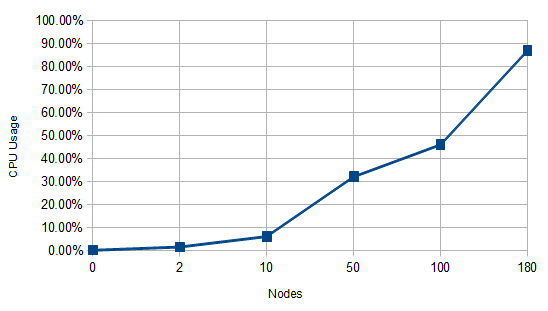
\includegraphics[width=11cm]{cpu_nodes.png}
\end{center}
\caption{CPU usage with increasing number of nodes}
\label{cpu_usage}
\end{figure}  


\section{Future Plans}

\subsection{Design}
As was mentioned in the project overview, some of the issues with the file-system design have not yet been addressed. 

First of all, there is still no clear plan on how to ensure data durability, as many nodes in the network will often go offline. The current plan is to rely on data redundancy and store file replicas on a number of nodes in the Chord ring after the successor of the node which was returned by the query. 
This would improve file downloading speed when querying the network for a specific file, as the DHT will be able to measure the latency to each of the nodes carrying the replica, and pick the fastest node for downloading.
It should also be noted that the number of nodes that should carry the replicas has not yet been determined, and a number of experiments will need to be executed to find a suitable value. These experiments have also not yet been designed.

Secondly, not all copies of the file currently in the network are going to be up-to-date. To ensure that the user always receives the most recent copy, when performing a lookup, a weighted voting scheme will need to be introduced. The replicas will be assigned a version number, and each replica of a file will be assigned a certain number of votes. Whenever the file is accessed, or written to, a certain number of $r$ votes to read a file, and a certain number of $w$ votes to write a file will be collected, such that $r + w$ is more than the total number of votes assigned to file.  
This mechanism should guarantee that any lookup will always retrieve the most recent version of the file \cite{versioning}, however, the implementation details of the mechanism are not yet finished. 

Next, no decision has yet been made on how the filesystem will deal with free space limits on machines running the nodes. Ideally, filesystem users should be asked how much space they want to assign to the filesystem, and the files stored on their drives should be prioritized, depending on whether the user owns the file, or whether it's a commonly accessed file. The files with high priority could then be maintained on the user's drive, while files with low priority could be overwritten if a request from the DHT is routed to the user's node. 

In addition, the implementation details of the FUSE interface need to be made more concrete, as it is not entirely clear what methods of the DHT interface FUSE operations will map to, and how they will interact with the index file.

Finally, distributed peer-to-peer filesystem literature still needs to be consulted regarding the presence of malicious nodes in the network. 

\subsection{Implementation}

On the implementation side, the current goal of the project is to finish implementing a suitable Chord prototype. Once that is done, and the design issues have been addressed, DHash and the FUSE interface to the filesystem will need to be implemented. At that point the filesystem will be in the state where the Andrew benchmark can be executed on it, thus making it possible to compare the speed of the filesystem to other filesystems. This will make it clearer as to how well it scales when nodes are added/removed, and what its most significant short-comings are, in regards to other similar filesystems.

An overview of the workplan is available in figure~\ref{milestones}.

\begin{figure}
\begin{tabular}{ | p{0.65\textwidth} | p{0.35\textwidth} | }
\hline
\textbf{Task} & \textbf{Dates} \\
\hline
Exam Period & April 8th 2013 - May 30th 2013 \\
\hline
Finish implementing Chord and DHash for the Twisted Python framework & June 1st 2013 - July 30th 2013 \\ 
\hline
\hline
{\bf Milestone: Chord and DHash layers implemented} & August 1st 2013 \\
\hline
\hline
Implement the simple security scheme on top of the DHash layer & August 1st 2013 - August 15th 2013 \\
\hline
Implement the FUSE interface to the filesystem. & August 15th 2013 - September 15th 2013 \\
\hline
Determine if there are any missing parts in the filesystem that prevent the Andrew benchmark from running, and implement them & September 15th 2013 - September 30th 2013 \\
\hline
\hline
{\bf Milestone: Andrew benchmark running} & 1st October 2013 \\
\hline
\hline
Compare Andrew benchmark results to other similar filesystems, determine if there are any shortcomings and devise a plan on how to overcome them & October 1st 2013 - October 15th 2013 \\
\hline
? & 15th October 2013 - 30th December 2013 \\
\hline
? & 1st January 2014 -  30th January 2014 \\
\hline
? & 1st February 2014 - 28th February 2014 \\
\hline
\hline
{\bf Milestone: Project finished} & 1st February 2014 \\
\hline
\hline
Write dissertation & 1st February, 2014 - 3rd April 2014 \\
\hline
Create presentation & 4th April 2014 - 30th April 2014 \\
\hline
\end{tabular}
\caption{Project timetable}
\label{milestones}
\end{figure}



%SHIT LEFT TO COVER:
%overwriting files?
%
%introduction
%workplan
%
%main problem with infinit: evaluation does not deal with churn

% As such, each user maintains a file list, of all files in
%the system that belong to the user.
%The current approach is to disregard all access control, and solve the issue later.
%
%
%% could copying be implemented in a clever way? how do other filesystems do it?
%\section{Purpose}
%
%The project will strive for:
%\begin{enumerate}
%\item simplicity, so that potential open source contributors find the project easy to grasp, thus enabling them to submit contributions;
%\item efficiency, since users will only consider the filesystem useful if it offers good performance.
%\end{enumerate}
%
%\section{Background}
%
%
%A list of decentralised peer-to-peer filesystems and their drawbacks follows:
%
%\begin{description}

%\section{Methods}
%
%And essentially no fully decentralised filesystem has been adopted by the wider public. 
%To build such a filesystem, a back-end and a front-end will be designed.
%
%The base of the back-end of such a system is a DHT (distributed hash table), capable of executing three commands among all nodes:
%The novelty of the system lies in being able to keep more files in the cloud, than there currently is space available on your physical hard drive. 
%
%This will be done by maintaining a list of the most frequently or recently used files that will be cached in the system, while leaving the rest of the space (that was allocated to the filesystem by the user) for keeping reconds of other people's files that they stored in the cloud.
%
%This should be possible, as the encouraged behaviour for a user of such a filesystem, is to allocate a large amount of hard drive space to it, but it is likely that the user will only use a small amount of that space for his or her own files (which are then going to be uploaded to this 'cloud' anyway).
%
%Describe how quorums are stored in the system,
%
%How we go from FUSE to executing all of the above (check FUSE API)
%
%Protocol needs to be scalable (as there might be a lot of nodes connected, how to address that?), also needs to support churn, as network nodes will move in and out of the network.
%
%Steps to editing a file:
%\begin{enumerate}
%\item user access a file on his/her filesystem
%\item retrieve(key) is called
%\item user edit and saves the file
%\item insert(key, value)
%\item update is propagated according to quorum rules
%\end{enumerate}
%
%Also need to address: security, persistence (how exactly am I adding sth new to the area)
%\begin{itemize}
%\item The back-end will be based on a DHT (Distributed Hash Table). 
%\item The front-end of the filesystem will be based on FUSE (Filesystem in Userspace) \cite{fuse}.
%\end{itemize}
%The implementation will target a real world workload. The ns-3 \cite{ns3} simulator will be used to test the implementation.
%
%\section{Current Progress}
%
%Work done so far consisted of a prototype implementation of the Chord protocol on top of the Python Twisted networking library, and a setting up of a testing infrastructure, capable of determining whether 
%\subsection{Network}
%\subsection{Replication}
%To enable reliable file storage, the peer-to-peer network must have a system of file replication. The most basic implementation is to store the exact same replica of the file at a fixed number of successor nodes. This is in fact the suggested method for higher level applications by Chord authors \cite{chord}.
%
%In the case that this is deemed inadequate during the development process, a more complicated scheme, such as Dynamic Replication could be implemented instead \cite{dhash}.
%

%\subsection{Cryptography}
%
%Unlike other Peer-to-peer systems such as Freenet, the emphasis of this project is not anonymity, but instead simplicity and efficiency. Only a minimal security mechanism will be provided, where the owner's files will be encrypted using a symmetric-key algorithm, with a possible candidate being Twofish (which is being widely used in a lot of products \cite{twofishprod}).
%This will not provide complete anonymity but will prevent unauthorised access to the user's files, as long as the key is kept safe.
%
%\subsection{Access Control}
%
%Providing an access control system is not in the scope of this project, and the task of implementing such a system is left to a higher-level application. However, an API will be provided in order to make this possible. 
%
%Since the contents of the files stored on the filesystem will be encrypted with the owner's key, this will to an extent prevent unauthorised access to users' resources.
%

%\section{Evaluation}
%
%As was mentioned, the implementation targets a real-world setup. However, due to limited resources, the simulator ns-3 \cite{ns3} will be used for specific test cases. This will allow for performing simulated experiments on systems involving a large number of nodes in order to determine how well the system scales, as well as performing real-world experiments with the intent of comparing performance to other well-established filesystems.
%
%\begin{itemize}
%\item Well-established and commonly used benchmarks in filesystem evaluation are the Andrew benchmark \cite{andrew}, and the Linux kernel build \cite{kernelb}. The results obtained from running these benchmarks would be compared to results presented in other filesystem papers.
%
%\item As it is common to compare the performance of peer-to-peer filesystems to the performance of NFS \cite{oceanstore} \cite{ivy} \cite{pastis}, a number of real world experiments would be structured upon simple operations executed on NFS, and a comparison would be produced.
%\end{itemize}
%
%\section{Outputs}
%
%A prototype of the system described will be made available as an open source project under the GPL \cite{gpl} license. The implementation will consist of a front-end and a back-end, providing full usage capabilities on any Linux-based operating system, as well as Mac OS X. Windows will not be supported, due to the lack of a mature port of FUSE. 
%
%The project will be published on a GitHub \cite{github} repository, and open to contributions from the open source community.
%
%\section{Workplan}
%
%The workplan timetable is given below (removed).
%
%As the project progresses, it is likely that changes will be made to the timetable.

\bibliographystyle{IEEEtran}
\begin{thebibliography}{10}
\bibitem{dropbox}
Dropbox. http://www.dropbox.com/
\bibitem{gdrive}
Google Drive. http://drive.google.com/start/
\bibitem{coral}
M. J. Freedman, E. Freudenthal, D. Mazieres.
Democratizing content publication with Coral.
In NSDI, Mar. 2004.
\bibitem{ns3}
ns-3. Discrete-event network simulator. http://www.nsnam.org/
\bibitem{chord} 
I. Stoica, R. Morris, D. Karger, M. F. Kaashoek, and
H. Balakrishnan. Chord: A scalable peer-to-peer lookup
service for internet applications. In Proceedings of the 2001
Conference on Applications, Technologies, Architectures,
and Protocols for Computer Communications, pages
149–160. ACM Press, 2001.
\bibitem{fuse}
FUSE: Filesystem in Userspace. http://fuse.sourceforge.net/ 
\bibitem{cfs}
F. Dabek, M. F. Kaashoek, D. Karger, R. Morris, and I. Stoica. Wide-area
cooperative storage with CFS. In SOSP, Oct. 2001.
\bibitem{oceanstore}
J. Kubiatowicz, D. Bindel, Y. Chen, S. Czerwinski, P. Eaton, D. Geels, R. Gummadi, S. Rhea,
H. Weatherspoon, W. Weimer, C. Wells, and B. Zhao. Oceanstore: An architecture for globalscale persistent store. In Proc. ASPLOS’2000, Cambridge, MA, November 2000.
\bibitem{ivy}
A. Muthitacharoen, R. Morris, T. Gil, and B. Chen. 
Ivy: A read/write peer-to-peer filesystem. 
In Proc. of OSDI, 2002.
\bibitem{towards}
J. Quintard. Towards a worldwide storage infrastructure.
PhD thesis, University of Cambridge, September 2010.
\bibitem{freenet}
The Freenet Project. https://freenetproject.org/
\bibitem{surveyofopenproblems}
R. Hasan, Z. Anwar, W. Yurcik, L. Brumbaugh, and
R. Campbell. A survey of peer-to-peer storage techniques for
distributed file systems. In ITCC �05: Proceedings of the
International Conference on Information Technology: Coding
and Computing (ITCC�05) - Volume II, pages 205�213,
Washington, DC, USA, 2005. IEEE Computer Society.
\bibitem{dhash}
M. Leslie.
Reliable Data Storage in Distributed Hash Tables. Oxford University. 2005.
\bibitem{versioning}
D. K. Gifford. Weighted Voting for Replicated 
Data. In Proceedings of the Seventh ACM 
Symposium on Operating Systems Principles, 
pages 159-159, December 1979
\bibitem{twofishprod}
Bruce Schneier. Products that use Twofish. http://www.schneier.com/twofish-products.html
\bibitem{andrew}
J. H. Howard. An Overview of the Andrew File System.
In Proceedings of the Winter USENIX Technical Confer-
ence, February 1988.
\bibitem{kernelb}
A. Traeger, N. Joukov, C. P. Wright, and E. Zadok. A
Nine Year Study of File System and Storage Benchmarking. ACM Transactions on Storage (TOS), 4(2):25–80,
May 2008.
\bibitem{pastis}
Busca, J. M., Picconi, F., \& Sens, P. (2005). Pastis: A highly-scalable multi-user peer-to-peer filesystem. Euro-Par 2005 Parallel Processing, 644-644.
\bibitem{gpl}
GNU General Public License. http://www.gnu.org/licenses/gpl.html
\bibitem{github}
GitHub. https://github.com/ 
\bibitem{chordalt}
Alternatives to the Chord Protocol. Boston University. http://nislab.bu.edu/sc546/sc441Spring2003/CallaMiraniCHORD/alternatives.html
\bibitem{andrewscale}
J. Howard, M. Kazar, S. Menees, D. Nichols, M. Satyanarayanan, R. Sidebotham, and M. West. Scale and performance in a distributed filesystem. ACM Transactions
on Computer Systems, 6(1), February 1988.
\bibitem{lxccont}
lxc Linux Containers. http://lxc.sourceforge.net/
\bibitem{p2plxc}
M. Bardac, R. Deaconescu, and A. M. Florea, ``Scaling Peer-to-Peer
Testing using Linux Containers'', in Proceedings of the 9th RoEduNet
IEEE International Conference, 2010, pp. 287-292.

\end{thebibliography}
\end{document}
